\chapter{Literature review}

This chapter should give the reader an overview of the components required for a global illumination model.
For the sake of the scope, one will briefly describe the different topics; therefore, if concepts or terms are unclear, one has to revise those accordingly.
As a side note, the order of sections does not correspond to the linearity of the concepts.

\section{Monte Carlo Integration}

In the book, \textit{Physically Based Rendering} \cite{pharr_physically_2017}, the authors explained that the integral, as a complex mathematical operator, opposes a challenge in computer science leading to numerous issues. 
Furthermore, they described that traditional methods like trapezoidal integration and the midpoint method are sufficient for low-dimensional and differentiable functions; however, these methods show a poor convergence rate for functions not fulfilling the criteria.
Nonetheless, approximations with numerical methods are the only solution to evaluate such terms due to the finite resources computers have.

Path-Tracing uses the Monte-Carlo integration because it has many practical properties presented later.
As with all Monte-Carlo techniques, illustrated by \cite{kalos_monte_2008}, it does use randomness for repeated random sampling to find an accurate solution on average.

Therefore, one gives a quick overview of probability theory to understand how the integration method works.

\subsection{Probability Theory}

A \textbf{random variable} is a function that maps a random process to a real-valued number, and one denotes it with a capitalised letter.
The \textbf{cumulative distribution function} $F(x)$ gives the probability for a random variable $X$ that is less than or equal to a value $x$.

\begin{align*}
F(X)=Pr\{X\le x\}
\end{align*}

Using calculus, one can differentiate $F(x)$, if possible, yielding the \textbf{probability density function} $f(x)$.
The density function describes the likelihood for a random variable to be in an interval $[a,b]$.

\begin{align*}
f(x)=\frac{dF(x)}{dx}
\end{align*}

The expected value is a weighted average, which is evaluable for a random variable.
This requires the cumulative distribution $F(x)$ and corresponding density function $f(x)$.

\begin{align*}
E[X]=\int_{\Omega}F(x)\,f(x)\,dx
\end{align*}

The final metric is the variance which gives the mean squared deviation.

\begin{align*}
V[X]=E\left[(x-E[x])^2\right]
\end{align*}

\subsection{Monte-Carlo Estimator}

Given is:

\begin{align*}
F=\int f(x)\,dx\quad\text{where}\quad f:D \mapsto R
\end{align*}

The task is to find an answer for the integral where $f(x)$ can take on any form.
The concept, as explained before, is to have a random variable $X:\Omega\rightarrow\mathbb{R}$ where $\Omega$ is a set of all possible outcomes mappable to a real-valued number.
Additionally, one assumes that samples are uniformly distributed over an interval $[a,b]$.
This result in the following estimator.

\begin{align*}
F_N=\frac{b-a}{N}\sum_{i=1}^{N}f(X_i)
\end{align*}

Currently, the estimator allows only for uniformly sampled values in an interval.
However, to generalise it, select a random variable with a probability density $p(x)$ that can weight $f(x)$.

\begin{align}
F_N=\frac{1}{N}\sum_{i=1}^{N}\frac{f(X_i)}{p(X_i)} \label{eq:mc-estimator}
\end{align}

Elaborating on eq.~\ref{eq:mc-estimator}, one can identify $F_N$ as a random variable which depends on the size of $N$, and $N$ sets the number of samples.
Note that $F_N \approx F$ and $F_N$ will be accurate on average.
One can show the accuracy with the expected value.

\begin{align*} 
E[F_N] &=E\left[\frac{1}{N}\sum_{i=1}^{N}\frac{f(X_i)}{p(X_i)}\right]\\
&=\frac{1}{N}\sum_{i=1}^{N}E\left[\frac{f(X_i)}{p(X_i)}\right]\\
&=\frac{1}{N}\sum_{i=1}^{N}\int_{a}^{b}\frac{f(x)}{p(x)}\,p(x)\,dx\\ &=\int_{a}^{b}f(x)\,dx 
\end{align*}

Now, one gives a quick overview of the advantages the integrations offers and quickly explains why these are useful.

In \cite{veach_robust_1997}, Veach pointed out essential advantages of the Monte-Carlo integration.
The first point mentioned was the convergence rate of the estimator.
He showed that the estimator converges with the rate of $O(N^{-1/2})$ for high dimensional integrals with discontinuities.
A vital attribute described in the thesis was that the convergence of an estimator with an infinity amount of variance is slow but guaranteed.
However, reducing the error by half requires four times more samples which opposes a problematic concern.
The second benefit is the simplicity of the algorithm.
He explained that this qualifies for flexible design with an integrator that is a black box.
This fact is essential as one can separate function from technical details.
The result is that the algorithm's implementation happens once, and the meaning of the data is unrelated, making it suitable for various problems requiring integration.
The last two traits are that Monte-Carlo can theoretically handle any domain, even an infinite-dimensional space, and work with integrands with singularities.

These benefits mentioned are the reason for the use of this method in computing light integrals.

\subsection{Optimisation}

The final part of the Monte-Carlo integration is about optimisations, as these play a considerable part in making this technique feasible for multiple applications.

The drawback of this technique is random sampling because the result depends on the number of drawn samples.
Consequently, a large sample count will produce more accurate results with a minor variance but increasing runtime.
The goal is to increase the efficiency of an estimator by reducing variance or runtime.

Before exploring techniques for variance reduction, one must clarify what efficiency means.

\begin{align}
\epsilon[F]=\frac{1}{V[F]\,T[F]}
\label{eq:estimator-eff}
\end{align}

Veach explained that one tries to find an estimator where variance and runtime are neglectable, and the eq.~\ref{eq:estimator-eff} describes this as a trade-off with $V[F]$ being the variance and $T[F]$ time required to determine $F$; \cite{veach_robust_1997}.
Accordingly, an estimator can become more efficient if it reduces runtime or variance.

\paragraph{Importance Sampling} has the principle to find a probability density function $p(x)$ which is similar to the integrand $f(x)$.
Optimally, the $p(x) \propto f(x)$ and considering equation eq.~\ref{eq:mc-estimator} it would give this configuration.

\begin{align*}
\frac{f(X_i)}{p(X_i)}=\frac{f(X_i)}{c\,f(X_i)}=\frac{1}{c} \Rightarrow F_N=\frac{1}{N}\sum_{i=1}^{N}\frac{1}{c}
\end{align*}

Leftover is a constant of proportionality $c$.
The proportionality of $p(x)$ and the current configuration of the summation demands that the normalisation must be the integral's value; \cite{veach_robust_1997}.

\begin{align*}
c=\frac{1}{\int\,f(x)\,dx}
\end{align*}

Based on that, the authors of the book \cite{kalos_monte_2008} conclude that a $p(x)$ similar to $f(x)$ will lead to a tremendous variance reduction.
The decrease is due to increasing the likelihood of sampling areas where the integrand is large, contributing more to the final result.
There are some constraints for $p(x)$ where it must match the behaviour of the integrand and its upper bound with $\forall x : p(x) > f(x)$.
Caution, selecting an incorrect $p(x)$ can have the opposite effect leading to more variance.

\paragraph{Adaptive sample placement} is another option to increase the efficiency of an estimator.
The basic idea is to sample more complicated or contributing regions based on previous samples.
However, the main disadvantage pointed out by \cite{veach_robust_1997} is the introduction of bias to the estimator that could lead, as an example, to image artefacts.

A quick excurse to elaborate on the problem of bias.

\begin{align*}
\beta = E[F]-\int f(x)\,dx
\end{align*}

It describes the difference between the expected value and the exact value of the integral; recall the original estimator fulfilled the property $E[F]=\int\,f(x)\,dx$ and is therefore unbias.
Nonetheless, as explained in \cite{kalos_monte_2008}, it does not matter if an estimator is biased if it helps by a significant amount with variance.

Russian roulette is one possible technique that can be incorporated well.
The technique intends to reduce sampling regions where the integrand is low as these contribute less to the final result.

In \cite{pharr_physically_2017} the authors elaborated that skipping low values does not matter because the expected value is still correct on average.
Another fact they explained is that Russian roulette does not reduce variance (it can even increase it), but it improves efficiency by not evaluating less important regions; hence runtime improves.

\section{Light Integrals}

Performing light transport simulations requires a formalisation of light.
For Path-Tracing, one utilises tools from physics to create a framework.
Duin \cite{duin_beleuchtungsalgorithmen_1993} described different models of light and how each of them comes with particular strengths in modelling the light's behaviour.
He elaborated that these models, like particle dualism, are outstanding in describing the nature of light but are not necessary for computer graphics where optics and radiometry are sufficient to model light at its core.
Based on that, he stressed the idea of light propagation and explained how light traverses the scene and interacts with other objects.
The scene is a formal description containing elements like an object, light rays, volumetrics and more. 

\subsection{Rendering Equation}

In 1986 Kajiya \cite{kajiya_rendering_1986} proposed the famous rendering equation that describes light propagation based on physics radiative heat transfer literature.
As a general geometrical optics approximation, its purpose is to evaluate the leaving equilibrium radiance at a point $p$ in the direction $\omega_o$ from all in-coming directions $\omega_i$ with a cosine term and $f(p, \omega_o, \omega_i)$ as the reflectance function.

\begin{align}
L_o(x,\omega_o)=L_e(x,\omega_o)+\int_{S^2}f_r(x,\omega_o,\omega_i)\,L_i(x,\omega_i)\,\left|\cos\theta_i\right|\,d\omega_i
\label{eq:rendering}
\end{align}

See that eq.~\ref{eq:rendering} is a recursive formulation where the in-coming directions are again integrals determined at other points in the scene.
That is why there is no immediate solution to the rendering equation; however, Ray-Tracing with Monte-Carlo integration, known as Path-Tracing, builds the foundation to solve such a simulation problem.

\subsection{Three-Point Form}

The current rendering equation is not suitable for deriving the path integral.
An additional step is needed to present an integral over areas, the so-called three-point form; \cite{veach_robust_1997}.
Therefore, one replaces all terms in the eq.~\ref{eq:rendering} containing a direction $\omega$, recall that $\omega=\widehat{x'-x}$.

\begin{align*}
L(x,\omega)=L(x'\rightarrow x)\quad\wedge\quad f_r(x,\omega_o,\omega_i)=f_r(x''\rightarrow x'\rightarrow x)
\end{align*}

The arrow emphasises the direction of light flow; \cite{veach_robust_1997}.
The next step is to change the integral domain over an area $A$, which also changes the integration variable, including the cosine term.
In \cite{kajiya_rendering_1986}, there are self-describing figures that show the configuration of the points and directions.

\begin{align*}
d\omega=\frac{|\cos\theta'|}{\|x'-x\|^2}dA(x') \Rightarrow |\cos\theta|\,d\omega=\frac{|\cos\theta|\,|\cos\theta'|}{\|x'-x\|^2}dA(x')
\end{align*}

However, this is not yet correct because two points must be visible.
The function $V$ is a visibility function that verifies that two points are from each other visible.
One utilises the visibility function and a factor of the previous equation for a geometry term $G$. If two points are not mutually visible, then the function is 0.

\begin{align*}
G(x'\leftrightarrow x)=V(x'\leftrightarrow x)\frac{|\cos\theta|\,|\cos\theta'|}{\|x'-x\|^2}
\end{align*}

If one substitutes all terms in eq.~\ref{eq:rendering} then one gets the three-point form.

\begin{align}
L(x'\rightarrow x)=L_e(x'\rightarrow x)+\int_{A}L(x''\rightarrow x')\,f_r(x''\rightarrow x'\rightarrow x)\,G(x''\leftrightarrow x')\,dA(x')
\label{eq:three-point}
\end{align}

\subsection{Path Integral}

The path integral is an alternative representation of the rendering equation that comprehensively explains detailed rendering characteristics.
Its introduction aims to assemble the foundation for a local sampling technique used in the implementation of this thesis.

Deriving the integral is intuitive as one can take the eq.~\ref{eq:three-point} and recursively replace the incoming radiance with the equation itself.
The most challenging part is rearranging the equation so one conceptually shows the pattern.
The next part will present the integral in multiple elements.

\begin{align}
L(x_1\rightarrow x_0)=\sum_{n=1}^\infty P(\bar{x}_n)
\label{eq:path-integral}
\end{align}

The equation \ref{eq:path-integral} represents the path integral.
It summates the radiance of all contributing paths, which gives the value obtained by the camera plane.
The summation is over an infinite domain where only the subset of paths with finite length is of interest.

\begin{align}
P(\bar{x}_n)=\underbrace{\int_A \int_A \dots \int_A}_{n-1}\left(L_e(x_n\rightarrow x_{n-1})\,T(\bar{x}_n) \right)dA(x_2)\dotso dA(x_n)
\label{eq:path-radiance}
\end{align}

Consequentially, eq.~\ref{eq:path-radiance} is the amount of radiance of a path $\bar{x}_n=x_0,x_1,\dotso,x_n$ with $n+1$ vertices.
It demands solving multiple nested integrals over areas.

\begin{align}
T(\bar{x}_n)=\prod_{k=1}^{n-1}f(x_{k+1}\rightarrow x_k\rightarrow x_{k-1})G(x_{k+1}\leftrightarrow x_{k})
\label{eq:path-throughput}
\end{align}

As explained by \cite{pharr_physically_2017}, the throughput expresses the fraction of received radiance from a light source.
This part is essential for the Monte-Carlo estimator as it explains how to keep track of the throughput state during the rendering process.

Now, one summarises the benefits before the subsequent section explains how the path integral incorporates the Monte-Carlo algorithm.

Veach \cite{veach_robust_1997} provided a detailed overview of the path integral's advantages.
The first point he described is that one can derive new rendering algorithms employing general-purpose integration techniques like importance sampling.
The second benefit is a geometric primitive, the path, which makes computation more comfortable.
Another benefit of working with paths is that they are more exact and complete regarding light transportations, as one uses the whole trajectory of light rather than distinct segments.
The construction of such paths is not limited to local information. 
That qualifies for an open selection process of path vertices.
Last, it provides a framework to work with the probability density of paths.

\section{Path Tracing}

Path tracing is a possible rendering algorithm to create synthetic images.
It uses ray tracing and Monte-Carlo integration to compute photorealistic images.
For this, it needs a formula that has to be solved.
One has now covered both, which allows the introduction of a local sampling technique to compute images.

A \textit{local sampling technique} is a method that constructs vertices of the path one at a time based on local information; \cite{veach_robust_1997}.
The easiest way is to sample directions regarding a probability density function.
One uses ray tracing to find the next vertex position.
This approach also solves the visibility problem, constructing only valid paths.
Of course, this strategy to find paths is not ideal but sufficient, making it a good choice; \cite{pharr_physically_2017}.

The only problem now is that one would sample paths using a solid angle and recollect that an angle's probability density is not the same as the probability density of an area.
Therefore, one has to make the conversion to calculate the correct probability of a path.

\begin{figure}[h]
\centering
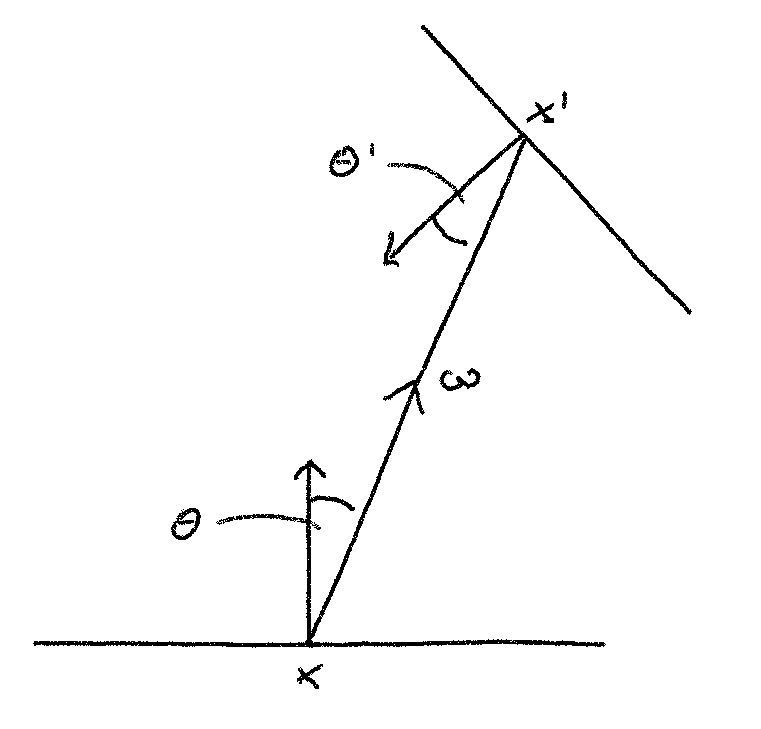
\includegraphics[width=0.33\textwidth]{sampling-configuration.png}
\caption[]{configuration of path vertices}
\label{fig:path-vertices}
\end{figure}

The figure \ref{fig:path-vertices} depicts the configuration of path vertices.
Vertex $x$ is the point of interest, and $x'$ is a potential successor.
In the current framework, one does sample a direction $\omega$ and cast a ray from $x$ towards $x'$.
Currently, one has only the probability of $\omega$. 
However, the following conversion term is applied to find the probability of $x'$.

\begin{align*}
p(x')=p(\omega)\frac{|\cos\theta'|}{\|x'-x\|^2}
\end{align*}

The authors of \cite{pharr_physically_2017} illustrated how integrating the probability density function in eq.~\ref{eq:path-radiance} causes the geometry function $G$ to partially cancel out with mentioned conversion.
However, be careful as the last vertex of a path is a light source.
This vertex originates from a distribution over the surface of the light.

\begin{align*}
\frac{f(x_{n}\rightarrow x_{n-1}\rightarrow x_{n-2})G(x_n\leftrightarrow x_{n-1})}{p(x_n)}\,\left(\prod_{k=1}^{n-2}\frac{f(x_{k+1}\rightarrow x_{k}\rightarrow x_{k-1})|\cos\theta_{k}|}{p(\widehat{x_{k+1}-x_{k}})}\right)
\end{align*}

Using eq.~\ref{eq:path-throughput} gives the final throughput term for the current use sampling framework.
Note that throughput is a combination of the reflectance function, the cosine and the probability of the incoming direction.

\subsection{Limitations}

As discussed in \cite{veach_robust_1997} path sampling is a simple and general method, but it has some limits.
Some paths do not have a correct sampling option, and even advanced approaches like bi-direction path tracing struggle with these paths.
There is also another category of ray tracing problems that are not solvable on Turing complete machines.

However, this does not oppose any problems as most paths are possible for simple scenes.
Nonetheless, see \cite{veach_robust_1997} for further details on that topic.

\section{Illumination Models}

In computer graphics, illumination models provide a specification to find the directional dependent radiance of a point; \cite{duin_beleuchtungsalgorithmen_1993}. 
An alternative name is the shading model because the purpose of such a model is to describe how a surface responds to light.
Due to that, it introduces multiple levels of darkness, colour and more which yields a three-dimensional-looking image.
One got already acquainted with a general illumination model, the rendering equation.

In \cite{duin_beleuchtungsalgorithmen_1993}, the authors mentioned three phases of shading models.
The last phase is interesting because it covers global illumination effects using optics.
Accordingly, models constructed based on optics are analytical models.

Next, one will present the Disney shading model \cite{burley_physically_2012}, \cite{burley_extending_2015}.
Burley and Walt Disney Animation Studios have designed a physically based shading model for the company's render with artistic controls in mind whilst preserving simplicity and robustness.
The motivation was to create numerous lighting options with correct surface responses across various environments and improve artist productivity.

\subsection{Principled Matrials}

Short overview of physically-based models.
-> What does this mean for modern illumination models.

Explain how Disney approached the design process of the new BSDF.
clarify what \textit{principle} means in the context of physically-based models

\subsection{Disney Bidirectional Scattering Distribution Function}

introduce to different types of light interaction
diffuse
specular
microfacet
Principled BSDF
Philosophy
construction of the shading model
